\documentclass[11pt]{article}
\usepackage[utf8]{inputenc}
\usepackage[T1]{fontenc}
\usepackage{graphicx}
\usepackage[export]{adjustbox}
\graphicspath{ {./images/} }
\usepackage{amsmath}
\usepackage{amsfonts}
\usepackage{amssymb}
\usepackage[version=4]{mhchem}
\usepackage{stmaryrd}

\begin{document}
Collateralized Mortgage Obligations

Collateralized mortgage obligations (CMOs) are an excellent example of a highly effective and somewhat simple use of structuring. CMOs assemble mortgage assets and finance those assets by issuing securities. CMOs divide the cash flows from assets such as mortgage pools or other mortgage-related products and distribute them with varying characteristics to different classes of security holders.

\section*{Prioritization of Claims within CMOs}
The key distinguishing feature between CMOs and other investment pools, such as mutual funds or the mortgage-backed securities discussed in the session, Real Estate Assets and Debt, is that CMOs use extensive structuring. Specifically, CMOs are financed with security classes or tranches that have substantially varied characteristics. A tranche is a distinct claim on assets that differs substantially from other claims in such aspects as seniority, risk, and maturity. Each tranche is typically tradable in units that may differ in size.

\begin{center}
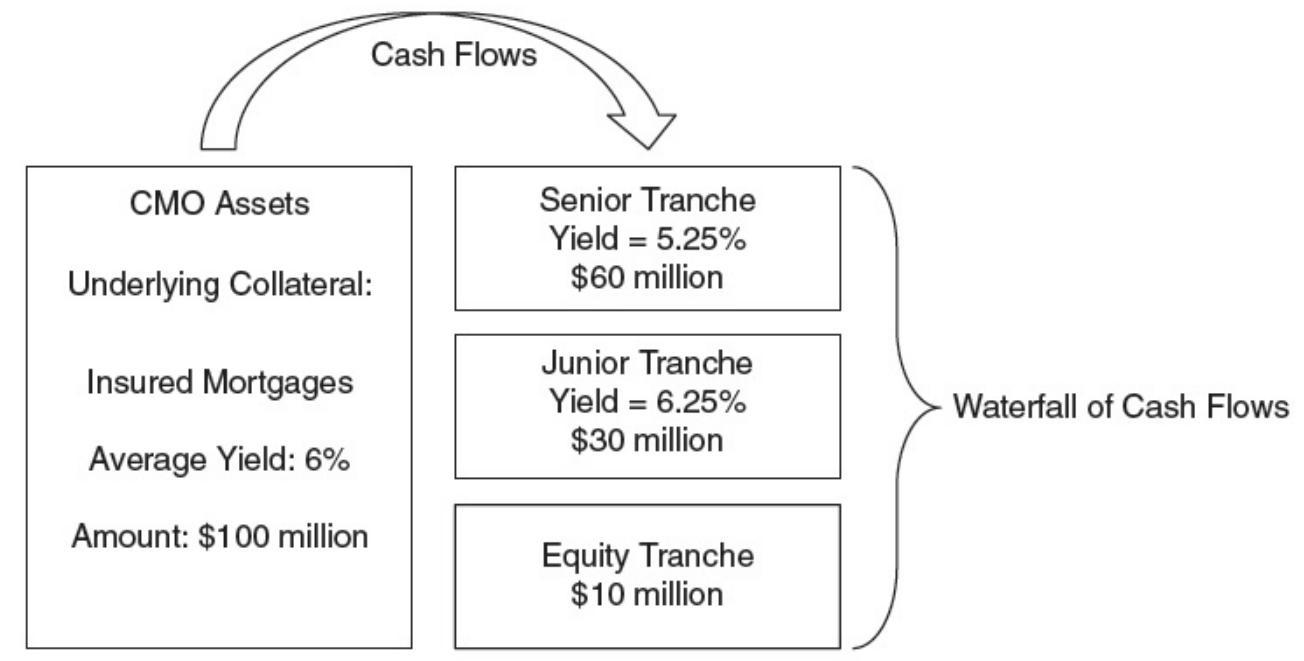
\includegraphics[max width=\textwidth]{2024_04_09_08813c5d5454963abf79g-2}
\end{center}

\section*{Simplified CMO Structure}
A CMO issuer structures these tranches to have different seniorities to the cash flows from the underlying mortgages. The exhibit above illustrates a stylized CMO structure for insured mortgages with only three tranches. In practice, CMOs usually have numerous tranches.

The assets on the left side of Simplified CMO Structure exhibit are often referred to as the collateral pool. The assets generate the cash inflows that are structured and distributed to the various tranches. In the case of insured residential mortgages, the structuring of the cash flows focuses on maturity and cash flow timing, because lenders bear little or no risk of principal losses due to mortgage defaults. In the case of commercial mortgages and subprime residential mortgages, the focus of the structuring of the cash flows from the mortgage pool is more on the allocation of default losses, since these loans are generally not insured.

The issuer of the CMO receives the monthly mortgage payments (principal and interest payments) from the collateral pool, and after collecting its fees, the issuer passes the payments on to the various tranches, following the procedures and priorities defined in the CMO prospectus. Each tranche has a coupon that it is promised and a prespecified priority in receiving distributions of principal payments.

\section*{Structuring of Sequential-Pay CMOs}
The sequential-pay collateralized mortgage obligation is the simplest form of CMO. In a sequential-pay CMO, each tranche receives a prespecified share of the interest payments based on each tranche's coupon and principal amount. Each tranche also potentially receives principal. When there is no default risk, it is the seniority to principal payments that is the focus of CMOs.

In the case of a sequential-pay CMO, the first-pay tranche (labeled as the senior tranche in the exhibit above) receives all principal repayments until the tranche's face value has been fully repaid. As a tranche's principal is paid down, its receipt of coupon payments is proportionately reduced. A tranche matures once it has received repayment of its entire principal value. The next senior tranche then receives the entire principal payments until it, in turn, matures. There is a final tranche, typically called the Z-tranche, that receives any residual cash flows.

The purpose to the structuring offered by a CMO is that it provides investors with a spectrum of risk-and-return opportunities. For example, an investor seeking shortterm, low-risk securities may purchase a highly senior tranche, while a longer-term investor might seek a tranche with a longer maturity, higher yield, and greater uncertainty of cash flow timing.

The structuring of the cash flows from the underlying mortgage collateral pools divides the prepayment risks (and, in other cases, default risks) of the pool into tranches that have low risk and tranches that have high risk. The higher-risk tranches can have extreme sensitivity to unexpected changes in prepayment rates (and, in some cases, default rates). Accordingly, the analysis and modeling of prepayment risks and default risks become even more crucial in the case of highly structured products.

In the case of insured residential mortgages, the exposure of each tranche to prepayment risk depends on the seniority of that tranche. The most senior tranches are virtually certain to mature quickly, regardless of prepayment rates. The tranches with the lowest seniority for receiving principal payments can have maturities that are extremely sensitive to prepayment rates. If interest rates increase, then prepayments by homeowners are likely to fall.

\section*{Longevity Characteristics of CMO Tranches}
Fluctuations in interest rates and other factors that drive mortgage prepayments cause a phenomenon known as extension risk. Extension risk is dispersion in economic outcomes caused by uncertainty in the longevity-especially increased longevity-of cash flow streams. For example, when interest rates rise, prepayment rates usually fall, and the life of most tranches, especially the more junior tranches, is extended, thereby increasing or extending the expected life of the tranche further than originally expected. In most CMO tranches, extension lowers the value. This reflects the general tendency of fixed-income instruments to fall in value when interest rates rise. However, some tranches can benefit from extension. These types of tranches might fall in value due to contraction when anticipated longevity declines. Contraction risk is dispersion in economic outcomes caused by uncertainty in the longevity-especially decreased longevity-of cash flow streams.

\section*{Estimating Cash Flows through a CMO Structure}
Consider a CMO with an underlying collateral pool of mortgages that generates $\$ 1,620,000$ of cash flow in its first month (after fees): $\$ 1,500,000$ in interest fees ( $9 \%$ annualized) and $\$ 120,000$ in principal repayments. A stylized sequential-pay two-tranche CMO structure is presented in the next exhibit. Payments are made first to Tranche A and then to Tranche B.

The next exhibit illustrates that, in month 1, both Tranche A and Tranche B receive their corresponding interest payments of $\$ 1,062,500(\$ 150,000,000 \times 8.5 \% / 12)$ for Tranche A and $\$ 437,500(\$ 50,000,000 \times 10.5 \% / 12)$ for Tranche B, for a total of $\$ 1,500,000$ in interest payments. In this simplified example, the interest payments received equal the interest payments owed to the two tranches, and there is no residual tranche. The remaining cash flow of $\$ 120,000$ is a principal repayment received from the underlying collateral, and it is used only to pay principal to Tranche A. The reason is that this is a sequential-pay two-tranche CMO, in which principal payments are made to Tranche A until the principal of Tranche A has been fully paid off, after which payments are made to Tranche B. Therefore, at the end of month 1, the principal balance for Tranche A is reduced to $\$ 149,880,000(\$ 150,000,000-\$ 120,000)$, and the principal balance of Tranche B remains at the initial $\$ 50,000,000$, since Tranche B received no principal payment.

START OF MONTH VALUES

Tranche A

Principal $=\$ 150,000,000$

Coupon $=8.50 \%$\\
Tranche B

Principal $=\$ 50,000,000$

Coupon $=10.50 \%$

\section*{TOTAL CASH FLOW FROM POOL}
\begin{center}
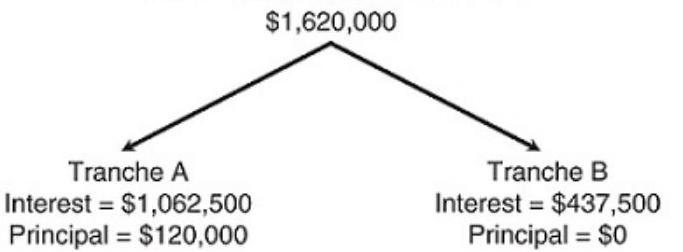
\includegraphics[max width=\textwidth]{2024_04_09_08813c5d5454963abf79g-3}
\end{center}

\section*{END-OF-MONTH VALUES}
Tranche A

Principal $=\$ 149,880,000$\\
Tranche B

Principal $=\$ 50,000,000$

\section*{Stylized Example of $\$ 1,620,000$ Cash Flow to a Sequential-Pay CMO with Two Tranches}
The mechanics of the payments in the following months will be similar. In the case of Tranche A, however, the interest payments due in the second month will decline because the total principal is decreasing with each principal repayment. For example, in the second month, Tranche A would be entitled to interest payments of only $\$ 1,061,650$ (\$149,880,000 principal at 8.5\%/12 interest).

The principal for Tranche B will start to be paid off only after the principal for Tranche A has been fully paid. If the prepayment rates of the mortgages underlying the CMO increase, Tranche A would be paid off faster and Tranche B would start to be amortized earlier. Conversely, if unscheduled principal repayments slow, the anticipated longevity of Tranche A will extend, but perhaps only modestly, as scheduled principal payments would presumably continue (i.e., extension risk would likely be minimal). However, the anticipated term of Tranche B could extend substantially. In this simplified example, Tranche B would continue until the last underlying mortgage made its final payment, and therefore, depending on prevailing rates and anticipated reinvestment opportunities, would likely be positively exposed to extension risk.

In actual CMO structures, there is typically an accrual tranche, or Z-bond, that receives no promised interest or coupon payments. Rather, the tranche serves as a residual, equity-like claimant, with rights to cash flows that remain after all fixed-income tranches have been satisfied.

\section*{Other CMO Structures and Tranches}
Numerous variations can be structured within a CMO issue other than the sequential-pay structure introduced in the previous section. This section highlights an important aspect of structuring: There is often an evolution that occurs in structured products wherein relatively simply structured products, if successful, evolve into increasingly complex and sophisticated products.

Here are several of the more popular types of CMOs.

Planned Amortization Class Tranches: Planned amortization class (PAC) tranches receive principal payments in a more complex manner than do sequential pay CMOs. Investors in some PAC tranches have high priority for receiving principal payments as long as the prepayment rates are within a prespecified range (the planned prepayment levels). When prepayments diverge from what was originally projected, the relative priorities of tranches can shift. In a sequential-pay structure, the relation between tranche longevity and prepayment rates is somewhat linear, meaning that each tranche's longevity to changes in prepayment speeds is somewhat stable at various levels of prepayment. But with PAC tranches, it is possible that a tranche will contract in longevity as prepayment rates accelerate to a certain point but then extend in longevity beyond that point. In other words, a tranche might have high priority to receiving principal payments in one range of prepayment speed and low priority if other prepayment speeds occur. Thus, PAC tranches can be riskier and more complex to analyze.

Targeted Amortization Class Tranches: Targeted amortization class (TAC) tranches receive principal payments in a manner similar to PAC tranches but generally with an even narrower and more complex set of ranges. The amortization procedures tend to identify narrower ranges of prepayment speeds within which tranches have particular priorities for receiving principal payments and interest. These prepayment ranges can be viewed more as targeted outcomes than as planned outcomes.

TAC tranches can be especially complex and risky. A sensitive TAC tranche can quickly switch from being quickly paid off to receiving no principal payments (and vice versa), even when prepayment speeds change by only a small amount.

Principal-Only Tranches and Interest-Only Tranches: Principal-only (PO) tranches receive only principal payments from the collateral pool, whereas interest-only (IO) tranches receive only interest payments from the collateral pool. Both tranches are therefore created by dividing cash flows from the mortgage collateral into the portion that is principal repayment and the portion that is interest. The principal repayment cash flows are distributed to one bond, the PO, and the interest cash flows are distributed to a second bond, the IO.

Investors in PO bonds are ultimately paid the face value of their bonds as borrowers eventually make the principal payments on their mortgages. The logic behind a PO is that investors buy these bonds at a discount from face value and eventually receive the face value through the scheduled principal repayments and prepayments received from the mortgages. PO tranches are positively exposed to extension risk in that their values decline when prepayments slow, since they receive no coupons.

An IO bond has a notional principal used to compute each interest payment. The cash flows received by investors in IOs decline as the principal is paid down. IO tranches are positively exposed to contraction risk in that their values decline when prepayments accelerate, since their payments are only interest because the notional principal is not repaid.

Prepayment sensitivity tends to be severe for POs and IOs, with one generally profiting when the other suffers. For example, in the case of POs on fixed-rate mortgages, when interest rates decline, the speed of prepayments typically accelerates. This contraction in longevity reduces the life of both the IO and the PO. PO tranches benefit from quicker receipt of their only cash flows: principal repayments in the fixed amount of the PO's face value. IO tranches suffer from principal reductions, since their only cash flows (interest payments) are proportionately reduced. On the other hand, when interest rates increase, the speed of prepayments declines, and the PO investor is paid the face value further in the future, lowering its effective return, while the IO receives a longer annuity of interest payments. Both tranches can be issued with adjustable- and fixed-rate underlying mortgages.

Floating-Rate Tranches: Floating-rate tranches earn interest rates that are linked to an interest rate index, such as the London Interbank Offered Rate (LIBOR), and are usually used to finance collateral pools of adjustable-rate mortgages. A collateral pool of adjustable-rate mortgages provides a stream of variable interest rate payments that can flow through to floating-rate tranches, which also have floating coupons. Floating-rate tranches can be structured to have rates that move more than the underlying index (e.g., twice the floating rate) or even in the opposite direction, which is known as an inverse floater tranche. An inverse floater tranche offers a coupon that increases when interest rates fall and decreases when interest rates rise. Floating-rate tranches can have specified upper and lower limits to their adjustable coupons.

\section*{Motivations of Structured Mortgage Products}
The primary motivations driving the demand for CMOs in the case of insured mortgages are summarized in the exhibit, Investor Motivations for Structured Products. Mortgages offer up to 30 years of coupons and principal payments, with high uncertainty regarding the level of unscheduled prepayments. Some investors prefer to take slices from this maturity range rather than invest in the entire range. Tranches permit investors to select securities that match their preferred exposures in terms of longevity and sensitivity to unscheduled prepayments.

As depicted in the next exhibit, these preferences are driven by two primary motivations: risk and return. Investors can lower their risk by selecting tranches with durations that match the duration of their liability stream. Cash flow matching is one of many risk-reducing strategies that can be facilitated by the structuring of claims.

Some investors have a market view of future interest rates or prepayment speeds. An investor can select tranches of CMOs that offer enhanced returns to the extent that the investor's market view is superior.

In the cases of both motivations in the next exhibit, the overall role being served by the CMOs is completion of the market. CMOs create numerous otherwise unavailable investment opportunities (i.e., tranches) from a pool of previously existing collateral. When the structuring is formulated in response to market demand, the enhanced set of opportunities facilitates improved portfolios from the perspective of the market participants.

\begin{enumerate}
  \item Risk management: Investors may be better able to manage risk through structured products.

  \item Return enhancement: Investors may be better able to establish positions that will enhance returns if the investor's market view is superior.

\end{enumerate}

\section*{Investor Motivations for Structured Products}
\section*{Valuing Default-Free CMOs}
The session, Real Estate Assets and Debt discusses unscheduled mortgage principal payments (i.e., prepayments). Prepayment decisions are made by property owners based on idiosyncratic events to the homeowners (e.g., job-related relocations) and macroeconomic factors, such as interest rates and housing prices. The Real Estate Assets and Debt session discusses the role of these unscheduled prepayment rates in driving the risks, returns, and values of residential mortgage pools.

The effect of prepayment speeds on the valuation of CMO tranches can be even more critical than the effects on the overall mortgage pools. The reason is that structuring creates tranches with varying risks. Suppose that overall mortgage values drop by $1 \%$ due to increased interest rates. Whereas collateral pools will tend to drop by $1 \%$, the losses to various tranches will vary based on the sensitivity of each tranche to interest rates. Long-term, highly sensitive tranches might drop by $5 \%$ or more, while very short-term tranches may be virtually unaffected. Some tranches, such as IO tranches, might even gain in value.

TAC, IO, and PO tranches can be especially sensitive to interest rates and prepayment speeds. Valuation of tranches requires careful and sophisticated analysis using advanced models of interest rates and prepayment speeds. The complexity of many CMOs creates both opportunities and threats. The sophistication of the models used to evaluate tranches creates the potential for analysts with superior skills to locate tranches of CMOs that are mispriced. However, the complexity of the\\
products and models also carries the danger that analysts with inferior skills will be induced into consistently making trading decisions that generate negative net present values. Highly complex tranches with innovative characteristics can appear to be attractively priced when they are actually overpriced; thus, the importance of due diligence cannot be overstated.

\section*{Systemic Risk and the History of Structured Mortgage Products}
There was a U.S. financial crisis involving CMOs on insured residential mortgages in 1994. Interest rates rose dramatically, causing most CMO tranches to extend in maturity as prepayment rates fell. The combination of extended maturities and higher interest rates caused market values of most tranches to fall, some quite severely. As investors and institutions suffered large losses, market liquidity eroded, and CMO tranches began to trade at prices reflecting even more conservative prepayment rate forecasts, further exacerbating the crisis.

Perhaps the worst case involved inverse-floating TAC tranches. Some of these tranches offered high coupons and were expected to mature within months at the end of 1993, due to high prepayment rates in the underlying mortgage pool and low interest rates. Therefore, these high-coupon and presumably short-term tranches traded at premium prices to their principal values and appeared to have little risk exposure to small or moderate interest rate changes. However, as part of a TAC structure, the tranches could experience dramatic shifts in seniority to principal payments if prepayment rates deviated from target ranges. In early 1994, prepayment speeds dropped such that the anticipated maturities of some of the TAC tranches extended from several months to many years, and switched from being the most senior to being the least senior tranches. Further, in the case of inverse floaters, the coupons on the tranches fell from high coupons to zero coupons as interest rates such as LIBOR skyrocketed.

The result was that some of the tranches, previously viewed by some market participants as having very low risk, fell from trading at premiums to trading at as little as $20 \%$ of face value by the summer of 1994 . This incredible drop in value occurred on tranche securities even though there was never a doubt that the principal value of the tranche would ultimately be recovered, since the underlying mortgage pool was insured by U.S. government agencies. Many institutions suffered huge losses, some firms collapsed, and the crisis widened until interest rates reversed their climb in the fall of 1994.

The prevalence and power of the structuring of mortgage products is often cited as causing or exacerbating both the financial crisis of 1994 and the financial crisis that began in 2007. In the most recent financial crisis, the financial losses in mortgage-backed structured products centered on default risk. In both cases, structured products contributed to increased systemic risk, substantially harming or even bankrupting major financial institutions and increasing uncertainty throughout financial markets.

Despite the past problems with structured mortgage products, the power of structured products has generated tremendous benefits. The long maturity and substantial prepayment risk of insured residential mortgages make unstructured ownership of mortgages undesirable to most market participants. Mortgages offer cash flows that range in maturity from 1 month to 360 months and offer uncertainty as to the size of each cash flow due to the prepayment options held by the borrowers. Relatively few market participants find mortgages to be attractive direct investments because of their range of scheduled cash flows and their exposure to prepayment rates and interest rates.

However, structured mortgage products allow market participants to select longevities and risk exposures that more closely align with their preferences. Thus, shorter-term fixed-income money managers can purchase short-term senior tranches, and longer-term managers, such as pension funds, can focus on longer-term tranches of insured mortgages. The emergence of structured mortgage products in the past several decades coincides with substantially reduced mortgage rate spreads, suggesting that structured products have enabled hundreds of millions of homeowners to enjoy substantially lower financing costs.

\section*{Commercial CMOs and Default Risk}
The previous sections discussed prepayment risk and extension risk. For CMOs with underlying portfolios of commercial mortgages or subprime residential mortgages, the primary risk is usually default risk. In CMO structures with substantial default risk, the primary result of the structuring of the cash flows is to vary the level of exposure of each tranche to default risk. The most senior tranches have the first right to scheduled and unscheduled principal payments and are last to bear losses from defaults. Conversely, the more junior tranches are highly subject to default losses from the underlying mortgage portfolio. The exposure of most CMO tranches to default risk is indicated by credit ratings assigned to each tranche.

As would be expected, credit ratings tend to differ quite considerably between the different tranches of a commercial mortgage-backed security (CMBS) because each tranche has different risk profiles, maturities, and subordination. Due to their subordination, more junior tranches have lower credit ratings. Conversely, senior tranches are often rated AAA because they have a high-priority claim on the cash flows and enjoy the extra security embedded by having initial default losses absorbed by the junior tranches.

The most junior tranches, often referred to as first-loss tranches, are often rated at non-investment-grade levels. This dispersion in credit risk exposure and credit ratings has the advantage of broadening the pool of appropriate investors. The senior, investment-grade-rated tranches are generally viewed as fixed-income securities, since they have limited expected exposure to default risk and are therefore primarily analyzed in the context of interest rate risk. In contrast, the most junior tranches are generally viewed and analyzed as risky securities substantially influenced by the risks of the underlying real estate rather than being influenced primarily by interest rate risks. Even a single large default can have a considerable impact on the performance of these junior securities. Therefore, in the case of CMBSs, junior tranches generally have higher coupons than senior tranches in the same structure. Particular attention is placed on the credit quality and other risk characteristics of the underlying mortgage pool, which is the collateral for the structure.

Default-risk CMO models focus on the expected rates of default, the correlation between defaults, and the losses on each defaulted issue. The idea is to forecast the probabilities of various cash flow streams from the underlying mortgage pool and to project the likelihood of payoffs to each of the tranches.


\end{document}